%%%%%%%% ICML 2023 EXAMPLE LATEX SUBMISSION FILE %%%%%%%%%%%%%%%%%

\documentclass{article}

% Recommended, but optional, packages for figures and better typesetting:
\usepackage{microtype}
\usepackage{graphicx}
\usepackage{subfigure}
\usepackage{booktabs} % for professional tables

\usepackage{tikz}
% Corporate Design of the University of Tübingen
% Primary Colors
\definecolor{TUred}{RGB}{165,30,55}
\definecolor{TUgold}{RGB}{180,160,105}
\definecolor{TUdark}{RGB}{50,65,75}
\definecolor{TUgray}{RGB}{175,179,183}

% Secondary Colors
\definecolor{TUdarkblue}{RGB}{65,90,140}
\definecolor{TUblue}{RGB}{0,105,170}
\definecolor{TUlightblue}{RGB}{80,170,200}
\definecolor{TUlightgreen}{RGB}{130,185,160}
\definecolor{TUgreen}{RGB}{125,165,75}
\definecolor{TUdarkgreen}{RGB}{50,110,30}
\definecolor{TUocre}{RGB}{200,80,60}
\definecolor{TUviolet}{RGB}{175,110,150}
\definecolor{TUmauve}{RGB}{180,160,150}
\definecolor{TUbeige}{RGB}{215,180,105}
\definecolor{TUorange}{RGB}{210,150,0}
\definecolor{TUbrown}{RGB}{145,105,70}

% hyperref makes hyperlinks in the resulting PDF.
% If your build breaks (sometimes temporarily if a hyperlink spans a page)
% please comment out the following usepackage line and replace
% \usepackage{icml2023} with \usepackage[nohyperref]{icml2023} above.
\usepackage{hyperref}


% Attempt to make hyperref and algorithmic work together better:
\newcommand{\theHalgorithm}{\arabic{algorithm}}

\usepackage[accepted]{icml2023}

% For theorems and such
\usepackage{amsmath}
\usepackage{amssymb}
\usepackage{mathtools}
\usepackage{amsthm}

% if you use cleveref..
\usepackage[capitalize,noabbrev]{cleveref}

%%%%%%%%%%%%%%%%%%%%%%%%%%%%%%%%
% THEOREMS
%%%%%%%%%%%%%%%%%%%%%%%%%%%%%%%%
\theoremstyle{plain}
\newtheorem{theorem}{Theorem}[section]
\newtheorem{proposition}[theorem]{Proposition}
\newtheorem{lemma}[theorem]{Lemma}
\newtheorem{corollary}[theorem]{Corollary}
\theoremstyle{definition}
\newtheorem{definition}[theorem]{Definition}
\newtheorem{assumption}[theorem]{Assumption}
\theoremstyle{remark}
\newtheorem{remark}[theorem]{Remark}

% Todonotes is useful during development; simply uncomment the next line
%    and comment out the line below the next line to turn off comments
%\usepackage[disable,textsize=tiny]{todonotes}
\usepackage[textsize=tiny]{todonotes}
\usepackage{float}

% The \icmltitle you define below is probably too long as a header.
% Therefore, a short form for the running title is supplied here:
\icmltitlerunning{Abstract Template for Data Literacy 2023/24}

\begin{document}

\twocolumn[
\icmltitle{Temporal and Spatial Exploration of Digital Crime in Germany}

% It is OKAY to include author information, even for blind
% submissions: the style file will automatically remove it for you
% unless you've provided the [accepted] option to the icml2023
% package.

% List of affiliations: The first argument should be a (short)
% identifier you will use later to specify author affiliations
% Academic affiliations should list Department, University, City, Region, Country
% Industry affiliations should list Company, City, Region, Country

% You can specify symbols, otherwise they are numbered in order.
% Ideally, you should not use this facility. Affiliations will be numbered
% in order of appearance and this is the preferred way.
\icmlsetsymbol{equal}{*}

\begin{icmlauthorlist}
\icmlauthor{Tim Gerne}{equal,first}
\icmlauthor{Tim Haigis}{equal,second}
\icmlauthor{Monica Janders}{equal,third}
\icmlauthor{Lukas Weber}{equal,fourth}
\end{icmlauthorlist}

% fill in your matrikelnummer, email address, degree, for each group member
\icmlaffiliation{first}{Matrikelnummer 5465398, tim.gerne@student.uni-tuebingen.de, MSc Machine Learning}
\icmlaffiliation{second}{5481789, tim.haigis@student.uni-tuebingen.de, MSc Cognitive Science}
\icmlaffiliation{third}{Matrikelnummer 5570379, monica.janders@student.uni-tuebingen.de, MSc Machine Learning}
\icmlaffiliation{fourth}{Matrikelnummer 5406074, lukas2.weber@student.uni-tuebingen.de, MSc Computer Science}

% You may provide any keywords that you
% find helpful for describing your paper; these are used to populate
% the "keywords" metadata in the PDF but will not be shown in the document
\icmlkeywords{Machine Learning, ICML}

\vskip 0.3in
]

% this must go after the closing bracket ] following \twocolumn[ ...

% This command actually creates the footnote in the first column
% listing the affiliations and the copyright notice.
% The command takes one argument, which is text to display at the start of the footnote.
% The \icmlEqualContribution command is standard text for equal contribution.
% Remove it (just {}) if you do not need this facility.

%\printAffiliationsAndNotice{}  % leave blank if no need to mention equal contribution
\printAffiliationsAndNotice{\icmlEqualContribution} % otherwise use the standard text.

\begin{abstract}

A significant portion of our routine actions is frequently carried out in the digital realm. Consequently, we explore whether this shift is not only apparent in lawful contexts but also observable in criminal activities. To this end we source datasets from the German Federal Office of Criminal Investigation due their supposed reliability and public availability.\\
After assesing data integrity and sufficiency, our two-fold analysis reveals a linear increase in cybercrime cases and high concentration in city states. We also observe a strong negative correlation between digital and analog fraud for the last ten years and discuss limitations of governmental data.

\end{abstract}


\section{Introduction}
\label{sec:intro}

After examining the available data thoroughly, we refrain from our initial idea of relating major events in Germany to crime rate development as the  German Federal Office of Criminal Investigation, known as the Bundeskriminalamt (BKA), does not provide datasets with sufficiently high spatio-temporal resolution. Instead we focus on long-term development of crimes and their regional differences.\\
We start by describing and examining the utilized datasets (Section~\ref{data_and_methods}). Then we segment our analysis into temporal and spatial aspects respectively, reflecting the structure of the data. We compare trends in cybercrime and conventional crime and attempt to analyze the development of computer fraud (Section~\ref{temp_analysis}). Cybercrime is defined by the BKA as: \textquotedblleft{}Cybercrime comprises criminal offenses that are directed against the Internet, data networks, information technology
systems and their data or which are committed using this information technology\textquotedblright{} \citep{BKA2014cybercrimedef}\footnote{\label{note1}Translated by the authors}. 
According to §263 of the German StGB \textquotedblleft{}Fraud penalizes individuals who, with the intention of gaining an unlawful financial advantage for themselves or others, damage another person's wealth by inducing or maintaining a misconception through the presentation of false facts or the distortion or suppression of true facts.\textquotedblright{} \citep{stgb_263}\footref{note1}
Additionally, we highlight regions characterized by high digital crime rates and provide comparisons of relevant geographic normalization methods (Section~\ref{spatial_analysis}). We conclude by discussing our findings and address limitations of the data (Section~\ref{sec:discussion}). 

\section{Data Assessment}\label{sec:methods}
\label{data_and_methods}

Utilizing data from the BKA, we have access to various datasets on criminal cases in Germany since 1987, consisting of annually compiled files. Although digital files from 1953 are available, their scanned format requires unreasonable effort for conversion into tabular files.
The data availability is increased since a 2012 system update by the BKA, including monthly case numbers for Germany and time series with annual overviews dating back to 1987.
Another update adds an annual distribution of cases across federal states, districts and cities, enabling a spatial analysis. Depending on the offense and analysis type, usable data dates back to 1987 or 2012, with some analyses starting in 2016 due to legal changes.\\
For further readability we introduce columns of common tables containing relevant information for this project. It is important to note that the exact naming of columns differs in some tables as the labeling and overall format changes over the years.\\
The annual federal tables \citep{PKS-Overview} \citep{BU-T01-2022} include the column \textquotedblleft{}Erfasste Fälle\textquotedblright{} containing registered cases on a number of crimes. Individual categories of crimes are encoded with numerical keys along with numerical group keys which aggregate multiple categories into a single key. The columns related to \textquotedblleft{}Tatortverteilung\textquotedblright{} are segmented into various ranges based on the population size of the areas where the crimes took place, serving as crucial data for our spatial analysis.\\
The monthly federal table \citep{BU-T08-2022} offers columns with monthly data for each year using similar keys as the federal base table. The \textquotedblleft{}Tatzeit unbekannt\textquotedblright{} column includes cases without a specific month attribution, while the column \textquotedblleft{}Anzahl Fälle insgesamt\textquotedblright{} contains the total number of cases in that year.\\
The annual state table \citep{LA-T01-2022}, compiled by the BKA, uses base tables from federal state police departments (LKA) like the annual federal table, grouping cases by federal state.

The PKS provides two tables containing regional information as well as sufficiently detailed crime keys: The national base table and the federal base table.
The former includes columns where the number of cases are grouped by population size of the region in which they were recorded. 
These regions are distinctly categorized by population, with labels such as $<$$20k$, $20k$-$100k$, $100k$-$500k$ and $>$$500k$.\\
The PKS provides no clear definition on what is considered a region. Looking at city states where all cases are recorded in the $>$$500k$-category, we can place a lower bound on the granularity of regions, but without official documentation it is impossible to reliably map geographical regions to number of inhabitants. For examples and potential solutions see our GitHub repository \citep{GitHubSpatial}.\\
The federal base tables avoid these issues altogether as they group cases by federal states. The downside of these tables is a lower data consistency, due to the the data being collected by each federal state's LKA independently.

\begin{figure}
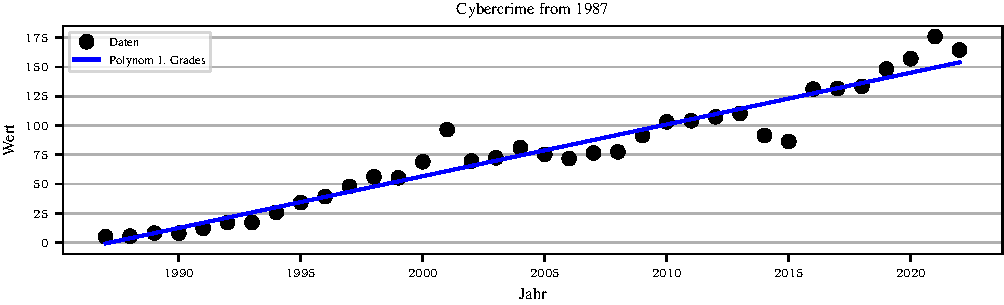
\includegraphics{fig/temporal_analysis_polynomial_fit.pdf}
    \caption{Development of cybercrime in Germany in absolute numbers. The method of least squares is used to fit a first degree polynomial with determination coefficient $R^2=0.930$.}
    \label{polynomial_plot}
\end{figure}
%
\section{Temporal Analysis}
\label{temp_analysis}
We first assess whether our different datasets with monthly and yearly crime cases match with regard to the absolute number of cases. We then conduct an analysis on the development of cybercrime and its subcategory, computer fraud, over the span of multiple years.

\subsection{Data Consistency}
\label{temp_data_consistency}
To check for consistency of the data within the monthly federal table, we sum up the monthly cases and the cases of the column \textquotedblleft{}Tatzeit unbekannt\textquotedblright{} for overall crimes and compared this sum with the column \textquotedblleft{} Anzahl Fälle insgesamt\textquotedblright{}. The values turn out to be identical for every year except for 2013 as there is no column \textquotedblleft{}Tatzeit unbekannt\textquotedblright{}. We assume that the missing column accounts for the higher value of \textquotedblleft{}Anzahl Fälle insgesamt\textquotedblright{} in this year as the difference has the same order of magnitude as the values of \textquotedblleft{}Tatzeit unbekannt\textquotedblright{} for the other years. \\
To ensure data consistency between the annual federal tables and the monthly federal tables we compare \textquotedblleft{}Anzahl Fälle insgesamt\textquotedblright{} from the former with \textquotedblleft{}Erfasste Fälle\textquotedblright{} from the latter. It is shown that the amount of cases in the annual federal table are consistently higher than the values from the monthly federal table. To find an explanation for these differences we subtract the number of attempted crimes from the overall crimes from the annual federal table. While this leads to a notable decrease in the number of total crimes it does not lead to the data of annually and monthly federal crimes being identical.\\
The annual federal table exhibits higher case numbers than the monthly federal table in certain years, while in other years, the relationship is reversed. For a visualization of the data discrepancy, please refer to \citet{GitHubTemporal}. The additionally provided information on the tables by the BKA do not lead to more insights on this discrepancy. For the scope of this project, it imposes a restriction on our ability to compare data from annually and monthly federal tables due to the unknown underlying 
differences in data collection.

\subsection{Data Analysis}
\label{temp_data_analysis}
%
\begin{figure*}[btp]
    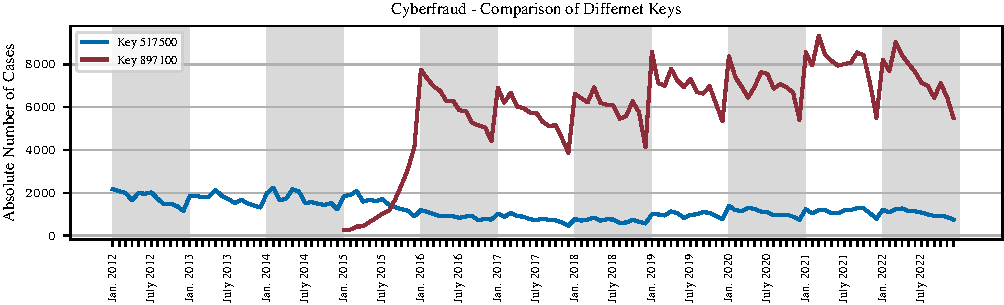
\includegraphics{fig/computer_fraud_from_diff_keys.pdf}
    \caption{Comparing the different keys encoding computer fraud, it can be seen that the later used key 897100 presents higher numbers than the initial key 517500. The only exceptions are the first few month after the new key is first introduced. The numbers differ by several orders of magnitude.}
    \label{fraud_plot}
\end{figure*}
%
An initial analysis of the development of cybercrime cases shows an increase between 1987 and 2022, which can be approximated by a polynomial of first degree with a coefficient of determination of $R^2 = 0.930$, shown in figure~\ref{polynomial_plot}. In our analysis, polynomial fittings of degrees two and three had just a slightly higher value for $R^2$ and show similarities to the linear trend. This development intrigued us to look for further interesting development of cybercrimes and how they compare to analog crimes. Due to the high difference in magnitude of conventional crime and cybercrime numbers, we decide to focus on a subset of crimes and corresponding cybercrimes: fraud and computer fraud.While cybercrime is only up to $\raisebox{-0.7ex}{\~{}}\, 3\%$ of overall crimes, computer fraud is up to $\raisebox{-0.6ex}{\~{}}\, 15\%$ of overall fraud. Therefore, a comparison of fraud and computer fraud seems more reasonable. For further insights we look at the case numbers of fraud and computer fraud on a monthly basis between 2012 and 2022.\\
While visualizing the monthly cases in figure~\ref{fraud_plot}, we encounter a change of keys indexing the cases of cybercrime. For the data between 2012 and 2015 the key 517500 is used for computer fraud and from 2016 onwards the same key is used for the crime computer fraud (other) (\textquotedblleft{}Computerbetrug (sonstiger)\textquotedblright{}). Furthermore, from 2015 onwards the key 897100 is used to track computer fraud. This key is not used before in the PKS. There is an overlap of the two keys for computer fraud for the year 2015, leading to the question which key to use to track computer fraud. As the BKA does not provide any guidance, we plot the development of both keys.
Initially there are lower values for the new key compared to the old key followed by a strong increase of the new key within the first year. The development of the initial key does not show any changes of magnitude over the years.


\section{Spatial Analysis}
\label{spatial_analysis}
After considering nation-wide data in the temporal analysis, we aim to dispel the implicit assumption of uniformly distributed crime rates with an exploratory spatial analysis. To this end we differentiate between regional differences at the expense of temporal scope and resolution, limiting ourselves to select yearly data. In the following we will first take a look at the available data, augment it with geographic information and compute two statistics for contrasted visualization.

The primary source for boundary data is based on the OpenStreetMap community \citep{geodata} and extended with current information on population and area per federal state by \citet{populationdata}.

\subsection{Spatial Methods}
\label{spatial_methods}

For the spatial data exploration we merge the LKA tables with the geographic data on federal states. In addition to the absolute number of cases provided by the table, we compute several relative statistics element-wise for each federal state:

The fraction of cybercrimes of all cases is calculated via
$$\text{\% cybercrime}:=\frac{\#\ \text{all cases}}{\#\ \text{cybercrime cases}} .$$
For years where regional numbers of cases are not officially provided in the table, we normalize the absolute number of cybercimes by the population size with
$$\text{cybercrime per capita}:=\frac{\#\ \text{cybercrime cases}}{\#\ \text{inhabitants}}\cdot100,000 .$$

The years 2016 and 2022 are selected for comparison to avoid issues with key changes and temporal anomalies based on findings from section~\ref{temp_analysis}.

\subsection{Spatial Results}
\label{spatial_results}
%
\begin{figure}[!h]
    \includegraphics{fig/spatial_analysis_3x2.pdf}
    \caption{(\textit{Top}) High number of cybercrime cases in North Rhine-Westphalia and Berlin along with general increase from 2016 (\textit{Left}) to 2022 (\textit{Right}). (\textit{Middle}) Strong increase of cybercrime ratio of all crimes particularly in Saxony-Anhalt. (\textit{Bottom}) Concentration of cybercrime in city states and Saxony-Anhalt defined by occurrence per 100k inhabitants.}
    \label{spatial_plot}
\end{figure}
%
The spatial distribution of cybercrimes is split into multiple categories and compared over two years in figure~\ref{spatial_plot}.
The first column shows data from 2016, while the second contains the most recent data from 2022. The general trend of overall increasing cybercrime rates is apparent in all shown statistics and correlates with the findings of the temporal analysis.\\
The first row shows the absolute number of cases, serving as baseline for further comparisons. Noteworthy is the overall high occurrence in North Rhine-Westphalia, Bavaria and Berlin. The second row highlights the relatively high cybercrime rate w.r.t.\@ all crimes in Berlin and a strong increase in Saxony-Anhalt, Hamburg and Bremen. The third row places particular emphasis on the difference between city states and larger federal states, as the number of cybercrimes per capita supersedes the latter by multiple orders of magnitude. In line with the trends in cybercrime rate, Saxony-Anhalt, Hamburg and Bremen display significant increases during this six year period.

\section{Discussion}\label{sec:discussion}
As there is little guidance provided by the BKA to help with the occurrence of key changes for computer fraud, we contacted an expert in this field, Prof.\@ Dr.\@ Jörg Kinzig, who serves as the Director of the Institute of Criminology at the Chair of Criminology, Criminal and Sanctions Law at the University of Tübingen. He redirected us to Benedikt Iberl, a doctoral candidate at the same institute. Among other insights, he informed us that as of January 2016, cybercrime is recorded using new underlying definitions, for what qualifies as cybercrime. Furthermore, based on the data he inferred the possibility that not only has the official definition of computer fraud changed, but also the internal categorization used by the BKA. He sent us an extract from the PKS stating that comparisons of any kind of fraud before and after 2016 are only possible to limited extent.\\
We fit the development of the absolute numbers of cybercrimes with a polynomial of first degree and compute $R^2 = 0.930$. This means it achieves a high variance explanation without overfitting. From further exploration in ~\citet{GitHubTemporal}, we see that the development of cybercrime in absolute numbers (as shown in figure~\ref{fraud_plot}) does not differ much from relative crime numbers, with nearly the same $R^2$ value for their linear approximation. \\
We see that the data points of 2014 and 2015 in figure~\ref{polynomial_plot} are far below the approximated line. The decrease in 2014 is explained in \citet{köppen2015cybercrime} which states that only cases are recorded, where the offense most likely took place in Germany. The reason for the increase in 2016 is based on the increase of computer fraud in this year. 
The graph of all crimes does not show such an obvious polynomial correlation, but there is a visible downwards trend that there is a downwards trend since about 20 years.\\
To find an approximation for the development of computer fraud cases is more difficult due to the legal changes and the corresponding discontinuity in the graph in 2016. We observed a negative correlation between the fraud cases and the computer fraud cases since 2016. \\
While North Rhine-Westphalia stands out in terms of absolute crime rates, it is also the largest federal state by population and thus insignificant when considering relative rates.
The reason for the observed concentration of cybercrime in city states and Berlin in particular remains unclear. We suspect this to be an artifact of the way reports are centrally collected, but a brief literature review revealed no additional insights.
However the high cybercrime rate in Saxony-Anhalt does not seem to be an artifact and might be worth investigating more closely in future annual reports.\\
Although we analyzed the trends mentioned above, we want to point out that the reliability of the provided data is not as high as we hoped in the beginning. \citet{köppen2015cybercrime} already referred to unreliable documentation and quoted a press release of the Federation of German Detectives: \textquotedblleft{}Citizens get the impression [when the PKS is published] that it is a statistical reflection of reality. Unfortunately, we are a long way from this. In fact, the statistics provide at best a very incomplete record of the work of the criminal investigation department.\textquotedblright{} \footref{note1}.
We hope these limitations inspire change in the overall approach to publishing and maintaining data of societal interest.

\section*{Contribution Statement}

Tim Gerne and Lukas Weber did temporal analysis and data assessment. 
Monica Janders did the mathematical analysis and plots.
Tim Haigis anlyzed and imported spatial data.

\bibliography{bibliography}
\bibliographystyle{icml2023}

\end{document}


% This document was modified from the file originally made available by
% Pat Langley and Andrea Danyluk for ICML-2K. This version was created
% by Iain Murray in 2018, and modified by Alexandre Bouchard in
% 2019 and 2021 and by Csaba Szepesvari, Gang Niu and Sivan Sabato in 2022.
% Modified again in 2023 by Sivan Sabato and Jonathan Scarlett.
% Previous contributors include Dan Roy, Lise Getoor and Tobias
% Scheffer, which was slightly modified from the 2010 version by
% Thorsten Joachims & Johannes Fuernkranz, slightly modified from the
% 2009 version by Kiri Wagstaff and Sam Roweis's 2008 version, which is
% slightly modified from Prasad Tadepalli's 2007 version which is a
% lightly changed version of the previous year's version by Andrew
% Moore, which was in turn edited from those of Kristian Kersting and
% Codrina Lauth. Alex Smola contributed to the algorithmic style files.
